\pagenumbering{Roman}
\setcounter{page}{1}
\lhead{Appendix \thesection}

\begin{appendix}
\section*{Appendix}
\phantomsection
\addcontentsline{toc}{section}{Appendix}
\addtocontents{toc}{\vspace{-0.5em}}

\section{IJulia}

\vspace{1em}
\begin{minipage}{\linewidth}
    \centering
    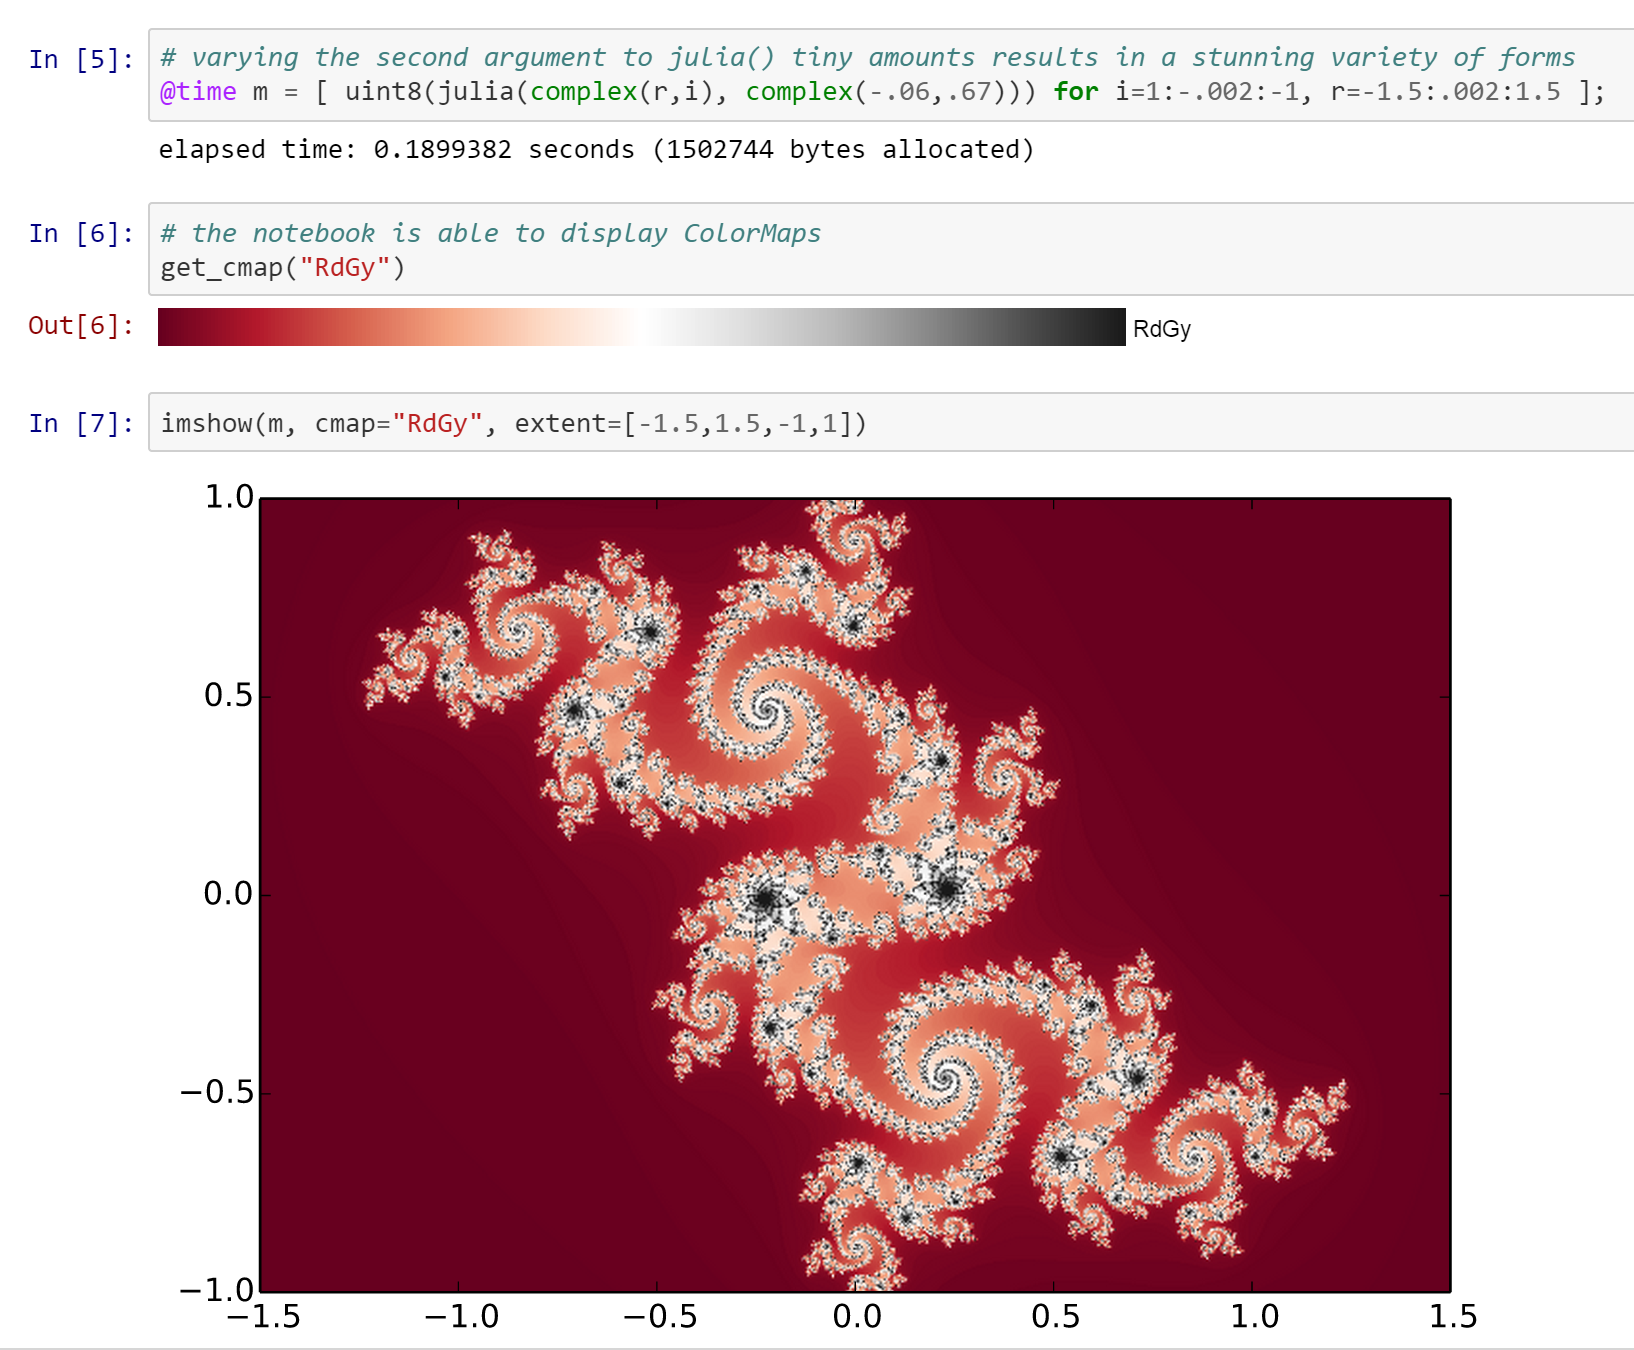
\includegraphics[width=0.9\linewidth]{graphics/ijnotebook.png}
    \captionof{figure}[IJulia Notebook Example]{
        Example of an IJulia Notebooks.
        Screenshot taken from \cite{IJuliaNotebook}
    }
    \label{fig:ijulianotebook}
\end{minipage}

\vspace{1em}
\begin{minipage}{\linewidth}
    \centering
    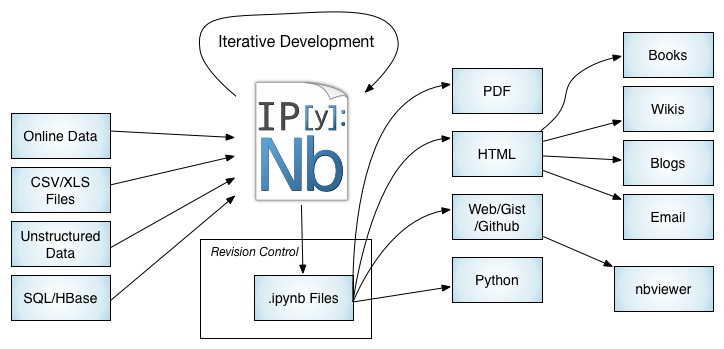
\includegraphics[width=0.9\linewidth]{graphics/IPython_Notebook_Workflows.png}
    \captionof{figure}[IPython Notebook Workflow]{
        Workflow of IPython Notebooks.
        Graphic from Wikipedia \cite{IPyhonNotebookFlow}
    }
    \label{fig:ipythonnotebookflow}
\end{minipage}
\section{Language Statistics}

All language statistics have been made with cloc \cite{CLOC} the current master of the github repositories.

\begin{table}[htbp]
    \centering
    \caption{Paraview, language statistic}
    \sffamily 
    \begin{longtable}{ l|l|l|l|l }
        \hline
        \textbf{Language}              &\textbf{files} &\textbf{blank} &\textbf{comments} & \textbf{code} \\
        \hline
        C++                            &2037          &70003         &86594         & 391121\\
        C/C++ Header                   &1937          &48345         & 93434        & 141581\\
        C                              & 273          &35843         & 17101        & 135937\\
        XML                            & 275          & 1930         &  3521        &  59030\\
        Fortran 77                     &  67          &   28         & 18039        &  39116\\
        Python                         & 209          & 5883         &  8719        &  21935\\
        CMake                          & 443          & 3705         &  6185        &  20025\\
        Javascript                     &  20          & 1285         &  1847        &   7982\\
        CSS                            &  23          &  750         &   251        &   4827\\
        HTML                           &  26          &  240         &  1692        &   2328\\
        JSON                           &  13          &    2         &     0        &   2162\\
        yacc                           &   1          &  207         &   138        &    881\\
        Bourne Again Shell             &  19          &  186         &   347        &    799\\
        make                           &   8          &  248         &    90        &    734\\
        Bourne Shell                   &  18          &  158         &   116        &    708\\
        XSLT                           &   3          &   46         &    17        &    388\\
        CUDA                           &   1          &   58         &   184        &    318\\
        Pascal                         &   2          &   69         &   102        &    228\\
        \hline
        SUM:                           &5375         &168986         &238377         &830100\\
        \hline
    \end{longtable}
    \normalfont
    \label{table:ParaviewStatistic}
\end{table}

\begin{table}[htbp]
    \centering
    \caption{VTK, language statistic}
    \sffamily 
    \begin{longtable}{ l|l|l|l|l }
        \hline
        \textbf{Language}&      \textbf{files}&\textbf{blank}& \textbf{comment}& \textbf{code}\\
        \hline
        C++                                   &3845         &203851         &179827        &1278279\\
        C                                     &1103         &130996         &289623        &707122\\
        C/C++ Header                          &3489         &103162         &246368        & 382728\\
        Python                                &1681         & 88983         &121122        & 258787\\
        Tcl/Tk                                & 573         & 11052         &  7830        &  48213\\
        CMake                                 & 739         &  4715         &  7424        &  35956\\
        Javascript                            &  47         &  6941         &  6747        &  33098\\
        CSS                                   &  33         &  1476         &   323        &  18100\\
        XML                                   &  10         &    17         &    36        &   8337\\
        Objective C++                         &  20         &  1210         &  1372        &   5601\\
        m4                                    &   3         &   660         &    83        &   4922\\
        yacc                                  &   3         &   726         &   570        &   4852\\
        HTML                                  &  25         &   553         &   531        &   4313\\
        Java                                  &  50         &   912         &  1192        &   4239\\
        Cython                                &  20         &   848         &  1625        &   3484\\
        Perl                                  &  11         &   939         &   950        &   3119\\
        JSON                                  &   3         &     5         &     0        &   2658\\
        Windows Resource File                 &  21         &   333         &   380        &   1835\\
        lex                                   &   3         &   215         &   162        &   1510\\
        DTD                                   &   3         &   435         &   477        &   1335\\
        Assembly                              &  13         &   202         &     0        &    936\\
        Bourne Again Shell                    &  16         &   191         &   333        &    866\\
        CUDA                                  &   6         &   113         &    77        &    740\\
        Bourne Shell                          &  15         &    64         &   122        &    380\\
        make                                  &   5         &    54         &   187        &    170\\
        IDL                                   &   1         &     0         &     0        &    150\\
        Windows Module Definition             &   3         &     3         &     0        &    142\\
        JavaServer Faces                      &   3         &    26         &     0        &     88\\
        Objective C                           &   2         &    13         &    18        &     17\\
        \hline
        SUM:                                 &11749         &558698         &867379        &2812005\\
        \hline
    \end{longtable}
    \normalfont
    \label{table:VTKStatistic}
\end{table}

\section{Romeo's GUI}

\begin{minipage}{\linewidth}
    \centering
    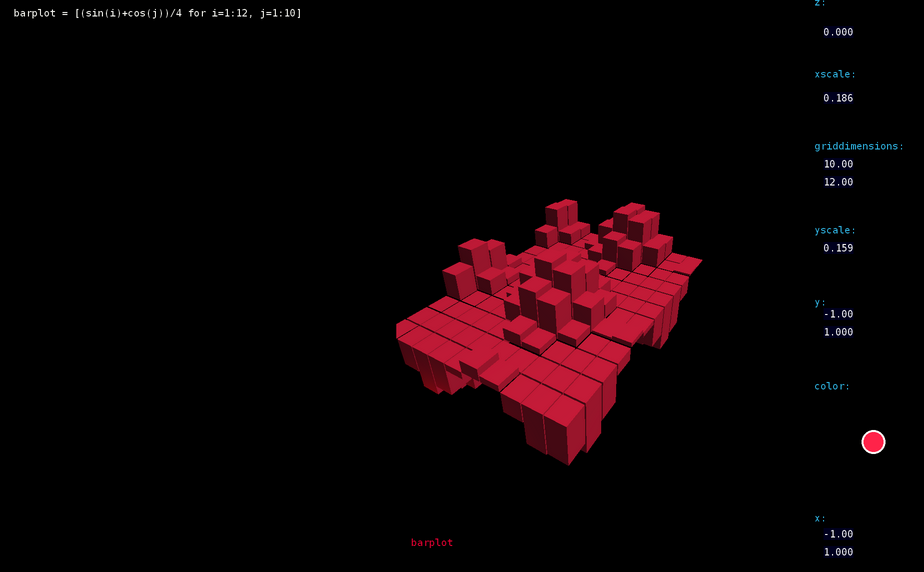
\includegraphics[scale=2.0]{graphics/screenshot.png}
    \captionof{figure}[Prototype]{Screenshot of the prototype. Left: evaluated script, middle: visualization of the variable barplot, right: GUI for editing the parameters of the visualization}
    \label{app:screenshot}
\end{minipage}

\section{Benchmark}

\begin{table}[htb]
\centering
\caption{FE Implementation comparison}
    \sffamily 
    \begin{tabularx}{1.0\textwidth}{l | c | p{5cm}}
        \hline
        implementations         & Language  & Speed in Seconds \\
        \hline
        JFinEALE                & Julia     & 9.6   \\
        Comsol 4.4 with PARDISO & Java      & 16    \\
        Comsol 4.4 with MUMPS   & Java      & 22    \\ 
        Comsol 4.4 with SPOOLES & Java      & 37    \\ 
        FinEALE                 & Matlab    & 810   \\
        \hline
    \end{tabularx} 
    \normalfont
    \label{table:FEComparison}
\end{table}


\end{appendix}
